\section{Análisis de la complejidad del problema}

El problema planteado por Scaloni es un caso específico del problema del 
Hitting-Set, cuya definición formal se presenta de la siguiente manera: dado un 
conjunto $A$ compuesto por $n$ elementos y $m$ subconjuntos $B_{1}, B_{2}, \dots, B_{m}$ 
pertenecientes a $A$ ($B_{i}\subseteq A \forall i \in \mathbb{N}_{m}$), se busca encontrar un conjunto $C \subseteq A$ tal que para cada 
subconjunto $C$, donde $C \subseteq A / \forall j \in \mathbb{N}_{m},  C \cap B_{j}\neq \emptyset$. 

Además de su formulación básica, el problema del Hitting-Set también presenta una versión
de decisión: dada la colección de un conjunto $A$ con $n$ elementos y $m$ subconjuntos
$B_{1}, B_{2}, \dots, B_{m}$ de $A$ ($B_{i}\subseteq A$ para cada $i$), junto con un 
parámetro numérico $k$, se plantea el interrogante sobre la existencia de un conjunto 
$C \subseteq A$ que cumpla con dos condiciones fundamentales:

\begin{itemize}
    \item En primer lugar, que la cardinalidad de $C$ sea menor o igual a $k$ ($\left| C \right|\leq k$) 
    \item En segundo lugar, que para cada subconjunto $B_{j}$, la intersección entre $C$ y $B_{j}$ no sea vacía ($C \cap B_{j} \neq \emptyset$) para todo $j$ perteneciente al conjunto de  números naturales hasta $m$.
\end{itemize}

El problema del Hitting-Set se sitúa en la clase de complejidad NP debido a su capacidad 
de verificación en tiempo polinomial, lo que implica una verificación eficiente de su 
solución propuesta. La verificación de la solución se reduce a confirmar dos condiciones 
fundamentales: Primero, se debe comprobar que la cardinalidad del conjunto propuesto $C$ 
es menor o igual a $k$, donde $k$ es un parámetro dado. Segundo, es necesario 
verificar que para cada conjunto $B_{j}$ dentro de una colección de subconjuntos 
$B_{1}, B_{2}, \dots, B_{m}$, $C$ contenga al menos un elemento de $B_{j}$.

Para realizar esta verificación, se llevan a cabo dos operaciones clave que definen la 
complejidad del proceso. La primera operación, relacionada con la verificación de la 
cardinalidad de $C$ ($\left| C \right|\leq k$), tiene una complejidad constante $O(1)$, 
ya que implica simplemente obtener el número de elementos en $C$ y verificar que $\left|C\right| \leq k$.

La segunda operación, que implica verificar la inclusión de al menos un elemento de $C$ 
en cada conjunto $B_{j}$, presenta una complejidad de $O(n \times m)$. Esto se debe a 
que para cada conjunto $B_{j}$ ($j$ perteneciente al conjunto de números naturales hasta 
$m$) (operación $O(m)$), se debe recorrer, en el peor de los casos, todo el conjunto $C$ 
($O(n)$) para verificar la pertenencia de al menos un elemento de este en $B_{j}$ 
(operación con complejidad $O(1)$ si tanto $B_{j}$ como $C$ se implementan como un conjunto 'set').

La clasificación del problema del Hitting-Set como NP-Completo se establece mediante la demostración
de su reducibilidad polinómica a partir de otros problemas ya catalogados como NP-Completo. 

En nuestro análisis, nos hemos propuesto abordar esta demostración de dos maneras distintas, 
empleando estrategias de reducción que ilustran la naturaleza NP-Completa del Hitting-Set Problem:

\begin{itemize}
    \item Reducción de Vertex Cover a Dominating-Set Problem -> Reducción de Dominating-Set Problem a Hitting-Set Problem.
    \item Reducción de Set Cover a Hitting-Set Problem.
\end{itemize}


Es importante destacar que la pertenencia de Vertex Cover y Set Cover a NP-Completo fue demostrada en clases anteriores.
\begin{itemize}
    \item  Vertex Cover [link]
    \item Set Cover [link]
\end{itemize}


\subsection{Reducción Vertex Cover a Dominating-Set Problem}

\begin{itemize}
    \item Vertex Cover: Dado un grafo $G=(V,E)$, donde V es un conjunto de vértices y $E$ es un conjunto de aristas, un Vertex Cover de G es un conjunto C \in V tal que para cada arista $(u,v)$ en $E$, al menos uno de los extremos de $u$ o $v$ esrá en $C$. Es decir, para cada arista en el grafo, al menos uno de sus extremos pertence al conjunto $C$. 
    \item Dominating Set: Dado un grafo $G$, se busca un conjunto de vértices $C$
    tal que, para todo vértice $v \in G$, este esté contenido en $C$ o existe al menos un vértice en $C$ adyacente de $v$.
\end{itemize}

La reducción $\text{Vertex-Cover} \leq _{p} \text{Dominating-Set}$ consta en lo siguiente:
Dado del grafo $G$ con $n$ vértices y $m$ aristas del problema Vertex Cover, para cada par de 
vértices adyacentes $v-w$, se agregan ambos al grafo $G'$ (del problema Dominating Set) junto a 
su arista y se agrega un tercer vértice auxiliar $vw$, adyacente a los otros dos. $A$ será el 
conjunto de vértices auxiliares. 

Luego, del conjunto $V'$ de $k$ vértices solución de Dominating Set, se debe agregar a $V$ (solución de Vertex Cover) todos los vértices de $V'$ que no estén en el conjunto de auxiliares y, para cada vértice en $V' \cap A$ se agrega a $V$  cualquiera de sus adyacentes. La primera parte de la reducción es $O(m)$ y la segunda es $O(k),k \leq n$, por lo que la complejidad total es $O(m+k)$, que es polinomial.

\[\text{Vertex-Cover} \leq _{p} \text{Dominating-Set}\]

\subsusbsection{Ejemplos:} 
\begin{figure}[H]
    \centering
    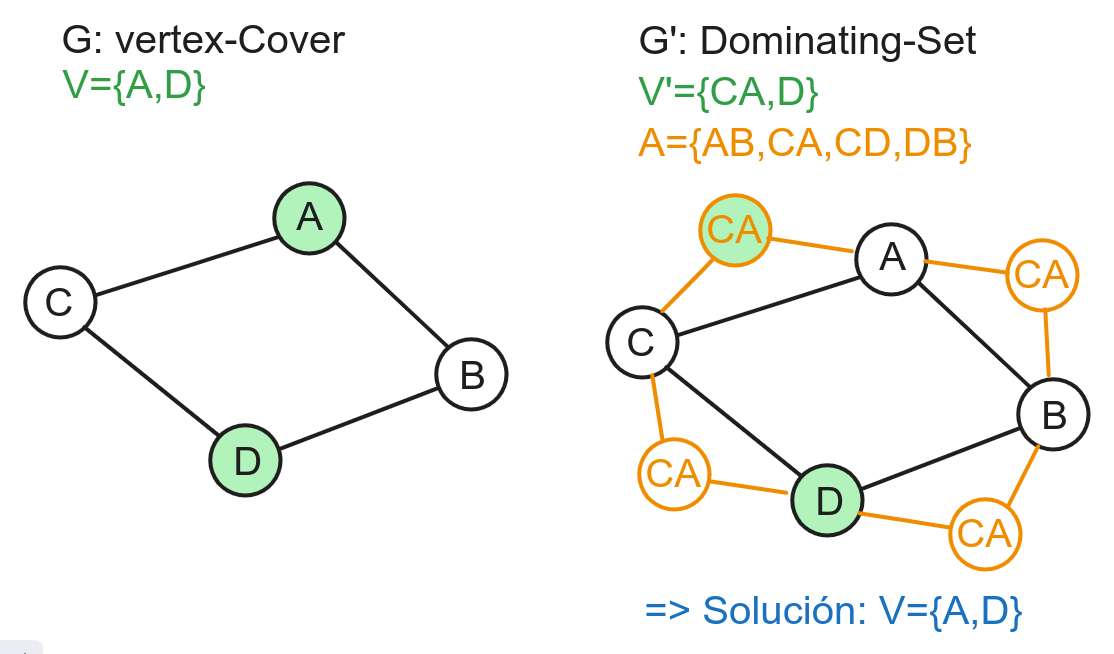
\includegraphics[width=0.8\textwidth]{img/ejemplo1_VC-DS.png}
    \caption{Ejemplo 1 de reducción de Vertex-Cover a Dominating-Set}
    \label{fig:ejemplo1_VC-DS}
\end{figure}

En el contexto del primer ejemplo analizado, se observó que los vértices incluidos en la solución proporcionada por el algoritmo de Dominating-Set formaban parte del conjunto inicial de vértices del problema Vertex Cover. 

\begin{figure}[H]
    \centering
    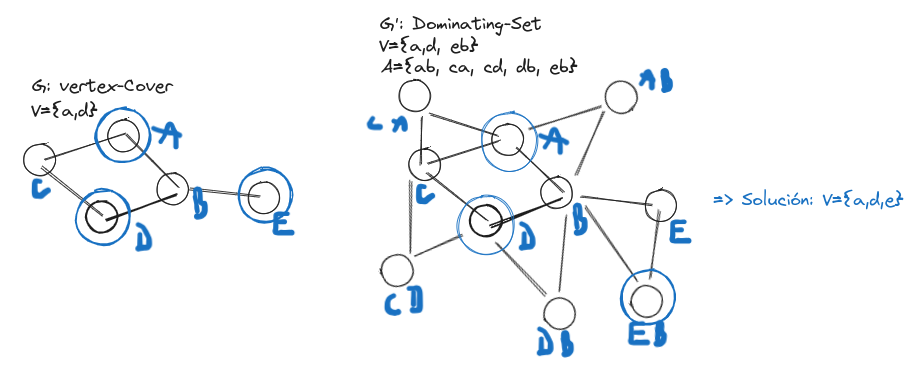
\includegraphics[width=0.8\textwidth]{img/ejemplo2_VC-DS.png}
    \caption{Ejemplo 2 de reducción de Vertex-Cover a Dominating-Set}
    \label{fig:ejemplo2_VC-DS}
\end{figure}

En constraste, en el segundo ejemplo analizado, se observó que no todos los vértices incluidos en la solución proporcionada por el algoritmo de Dominating-Set formaban parte del conjunto inicial de vértices del problema Vertex Cover ($eb$ es parte de la solución proporcionada por Dominating-Set).
Por ello, se optó por seleccionar un vértice adyacente al vértice $eb$, siendo el vértice $e$ la elección específica en la ilustración proporcionada.

Finalmente:

\[
    \begin{array}{c}
        \begin{split}
            \text{Vertex-Cover}  & \leq _{p} \text{Dominating-Set} \\
            \text{Dominating-Set}  & \leq _{p} \text{Hitting-Set} \\
        \end{split}
        \quad \overset{ \text{por transitividad} }{ \implies  } \quad
        \text{Vertex-Cover}  \leq _{p} \text{Hitting-Set} \\ \\
        \implies \text{Hitting-Set} \in \text{NP-Completo}    
    \end{array}
\]

\subsection{Reducción Dominating-Set a Hitting-Set}

La reducción $\text{Dominating-Set} \leq_{p} \text{Hitting-Set}$ consta en lo siguiente:
Dado un grafo $G$ de $n$ vértices del problema Dominating Set, para cada vértice $v_{i}$, se construye un grupo $B_{i}$ con él mismo y todos sus vértices adyacentes. Esto tiene un costo temporal de $O(N \times E)$, ya que para cada vértice $v_{i}$ se deben obtener los vértices adyacentes a $v_{i}$ y crear los conjuntos $B_{i}$ por cada uno de ellos (es decir, realizamos operaciones polinomiales para transformar nuestro problema de Dominating-Set a Hitting-Set). 

A su vez, esta reducción se caracteriza por ser de equivalencia simple ya que el resultado devuelto por el algoritmo de Hitting Set coincide directamente con los resultados esperados por el algoritmo de Dominating Set. Como consecuencia, no es necesario realizar operaciones adicionales o suplementarias para obtener el resultado deseado.


La complejidad del mismo se formula a continuación:
La construcción de los $m$ conjuntos $B_{i}$ es $O(N \times E)$. Ya que para cada vértice $v_{i}$ se deben obtener los vértices adyacentes a $v_{i}$ y crear los conjuntos $B_{i}$ por cada uno de ellos. 

\[\text{Dominating-Set}  \leq _{p} \text{Hitting-Set}\]

\subsusbsection{Ejemplos:} 

\begin{figure}[H]
    \centering
    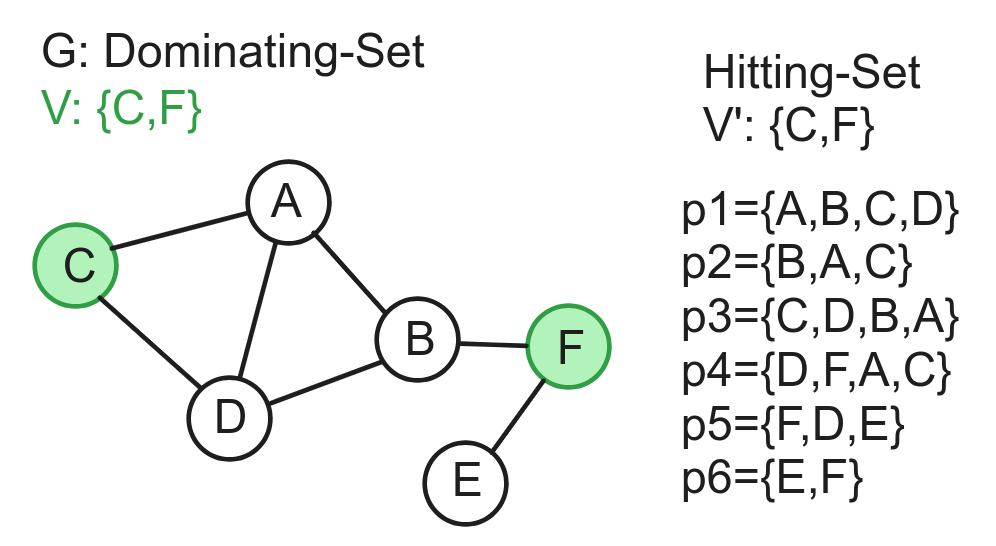
\includegraphics[width=0.8\textwidth]{img/ejemplo1_DS-HS.png}
    \caption{Ejemplo 1 de reducción de Dominating-Set a Hitting Set}
    \label{fig:ejemplo1_DS-HS}
\end{figure}


\begin{figure}[H]
    \centering
    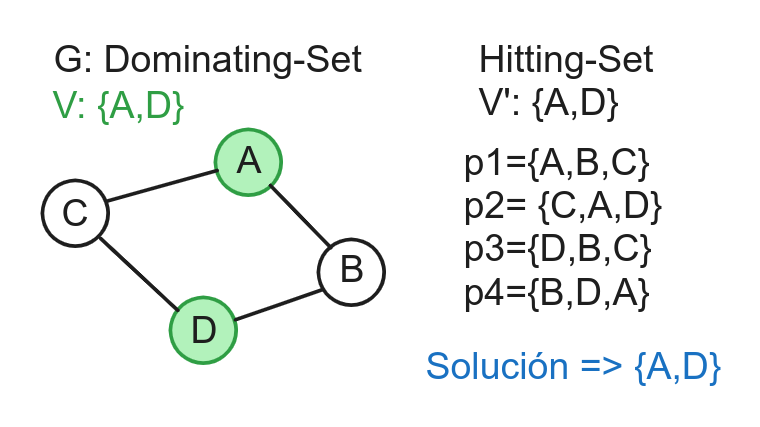
\includegraphics[width=0.8\textwidth]{img/ejemplo2_DS-HS.png}
    \caption{Ejemplo 2 de reducción de Dominating-Set a Hitting Set}
    \label{fig:ejemplo2_DS-HS}
\end{figure}


\begin{figure}[H]
    \centering
    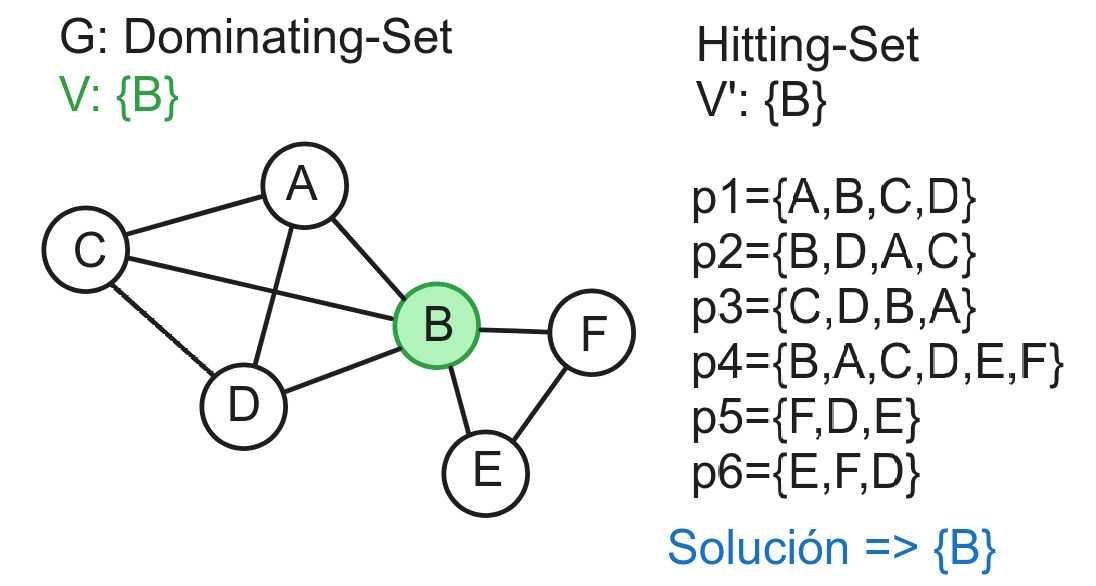
\includegraphics[width=0.8\textwidth]{img/ejemplo3_DS-HS.png}
    \caption{Ejemplo 3 de reducción de Dominating-Set a Hitting Set}
    \label{fig:ejemplo3_DS-HS}
\end{figure}

En los tres casos analizados, se evidencia que la solución derivada del problema Hitting-Set representa la solución óptima para el Dominating-Set.


\subsection{Reducción Set-Cover a Hitting-Set}

\begin{itemize}
    \item Set-Cover: Dado un conjunto finito $U$ y una familia $S= {S_1, S_2, ..., S_n}$ de subconjuntos de $U$, el problema de Set Cover consiste en identificar el menor número de conjuntos cuya unión aun contiene todos los elementos del universo. 
\end{itemize}

La reducción $\text{Set-Cover} \leq_{p} \text{Hitting-Set}$ consta en lo siguiente:
Dado un grafo $G$ de $n$ vértices del problema Set-Cover, para cada elemento del subconjunto $S_{i}$, se construye un grupo $E_{i}$ en el cual sus elementos van a ser cada $S_i$ en el cual está incluido. 

Esto tiene un costo temporal de $O(N \times U)$ (siendo $N$ la cantidad de subconjuntos $S$ y $U$ la cantidad de elementos del universo), ya que para cada subconjunto $S_{i}$ se debe recorrer sus elementos (en el peor de los casos todos tienen la misma cantidad que el universo) y crear los conjuntos $E_{i}$ (en caso de que no esté ya creado). En cada subconjunto nuevo $E_i$ se le agrega el $S_i$ donde está incluido, siendo esta una operación constante. 

El análisis del costo temporal asociado al problema del Set Cover se establece en O(N×U), donde N representa la cantidad de subconjuntos en S y U la cantidad de elementos presentes en el universo. Este costo se deriva de la necesidad de recorrer cada subconjunto S_i en la familia S y sus elementos correspondientes, operación que, en el peor de los casos, implica recorrer conjuntos de igual tamaño al universo.

Para cada subconjunto S_i, se realiza la creación de conjuntos E_i si no están previamente creados. En el proceso de generación de cada conjunto E_i, se añade el subconjunto S_i donde el elemento está incluido, siendo esta una operación de complejidad constante. 

De esta manera, realizamos operaciones polinomiales para transformar nuestro problema de Set-Cover a Hitting-Set. Además, al igual que la reducción de Dominating Set a Hitting Set, esta reducción se caracteriza por ser de equivalencia simple ya que el resultado devuelto por el algoritmo de Hitting Set coincide directamente con los resultados esperados por el algoritmo de Set-Cover. Como consecuencia de esta correspondencia entre los resultados, no es necesario realizar operaciones adicionales o suplementarias para obtener el resultado deseado.


\[\text{Dominating-Set}  \leq _{p} \text{Hitting-Set}\]

\subsusbsection{Ejemplos:} 

\begin{figure}[H]
    \centering
    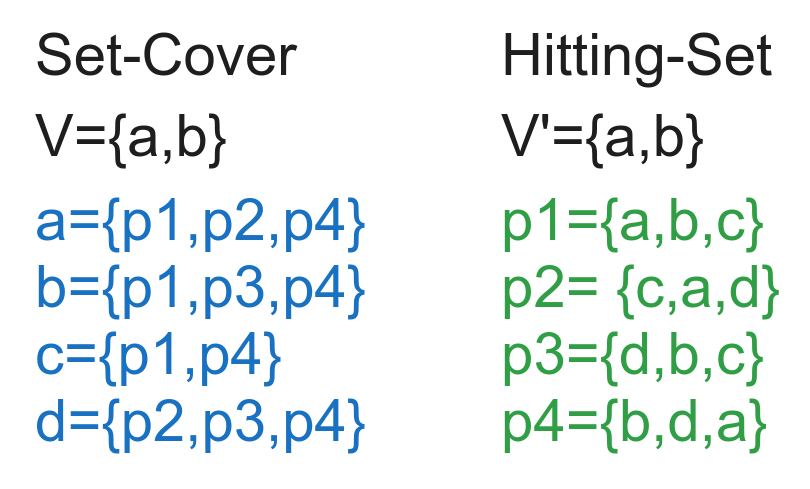
\includegraphics[width=0.8\textwidth]{img/ejemplo1_SC-HS.png}
    \caption{Ejemplo 1 de reducción de Set-Cover a Hitting Set}
    \label{fig:ejemplo1_DS-HS}
\end{figure}

\begin{figure}[H]
    \centering
    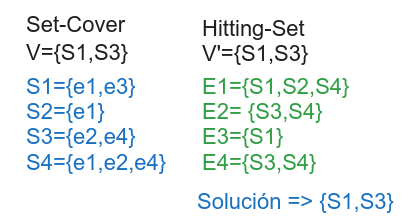
\includegraphics[width=0.8\textwidth]{img/ejemplo2_SC-HS.png}
    \caption{Ejemplo 2 de reducción de Set-Cover a Hitting Set}
    \label{fig:ejemplo2_DS-HS}
\end{figure}

Al igual que la reducción de Dominating-Set a Hitting-Set, en los dos casos analizados, se evidencia que la solución derivada del problema Hitting-Set representa la solución óptima para el problema de Set-Cover.




